\section{Introduction}
We have been doing experiments with Iris Plus 3DR\trademark quadricopters in the testing environment of the Smart Mobility Lab of KTH.
The environment is a $5\times5$ meter square area of 2 meters high.
Position of the agents are measured with the motion capture system Qualisys\trademark.
The velocity feedback and the plan are running on an offboard computer. And the transmission of the control inputs to the quadricopter is running at 35Hz through an RC link. The overall program is running with the ROS framework.
The computation of the abstractions and the plan solution of the problem are done offline (see digram \ref{diagram}).

\begin{figure}
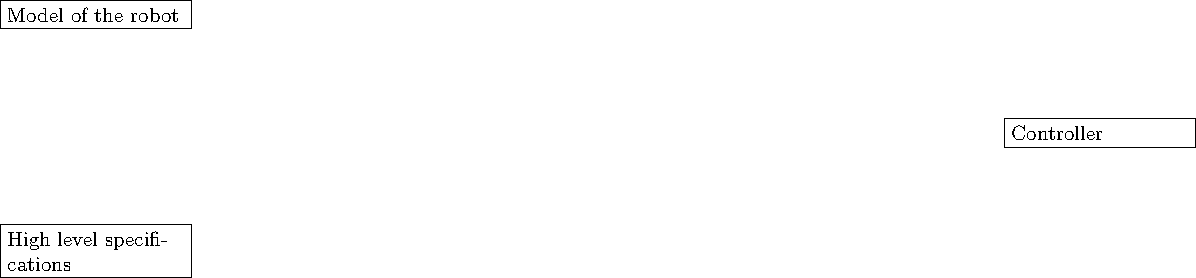
\includegraphics[width=\linewidth]{diagram.tex}
\label{diagram}
\end{figure}

Tests has been done on single agent (1 or 2 axis) and on multi agents.
Due to the state space explosion problem, we did not found any plans for some environments of too high dimensions (2D or multiagents).
The double integrator abstraction (without input memory) leads to models that were unusable in 2D. As well as the input extended state abstraction with 1 input memory could not be used with multi agent planning.
